\newcommand{\rsmpl}{\xleftarrow{\$}}

\newcommand{\alg}{\textsc{Alg}}

\newcommand{\ap}{\textsc{AccessPattern}}
\newtheorem{nonexample}[theorem]{Non-Example}


\section{Oblivious Sorting}

\begin{definition}
    An algorithm $\alg$ is \textbf{oblivious} if for all pairs of inputs $\mathcal{I}, \mathcal{I}'$ of equal length, we have:
    \[\ap(\alg, \mathcal{I}) \approx \ap(\alg, \mathcal{I}'), \]
where $\ap(\alg, \mathcal{I})$ denotes the observed access pattern when executing $\alg$ on input $\mathcal{I}$, and $\approx$ denotes two distributions are indistinguishable (either statistically or computationally, depending on the specific setting.)
\end{definition}

$ $

\begin{nonexample}
    QuickSort is \textbf{not} oblivious because it reads and writes array elements depending on the result of comparing with a pivot. These instructions leak information about the content of the input array.

    Consider the following two arrays: 
    \begin{center} 
 $Arr_1 := \begin{array}{|c|c|c|c|c|c|c|} \hline 
 7 & 6 & 5 & \textbf{4} & 3 & 2 & 1
 \\ 
\hline
\end{array}
$
 \[ Arr_2 := \begin{array}{|c|c|c|c|c|c|c|} \hline 
1 & 2 & 3 & \textbf{4} & 5 & 6 & 7
\\ 
\hline
\end{array}
\]

\end{center}

If in both $Arr_1$ and $Arr_2$, $\textbf{4}$ is picked to be the pivot, then QuickSort would move $Arr_1[0:2]$ to the right of $\textbf{4}$ while keeping $Arr_2[0:2]$ at the left of $\textbf{4}$. Therefore, one can distinguish the two inputs $Arr_1$ and $Arr_2$ by observing the different access patterns. 

\end{nonexample}

$ $

We can na\"ively compile QuickSort to be oblivious using $\textsc{PathOram}$. However, this incurs a log-squared (multiplicative) overhead. Since the runtime of QuickSort is $\mathcal{O}(n\log n)$ where $n$ is the input length, the resulting oblivious version of QuickSort runs in $\mathcal{O}(n\log^3 n)$.

In this lecture, we will see two direct constructions of oblivious sorting that achieve faster runtime than compiling QuickSort with ORAM. Our ultimate goal is to match the runtime of non-oblivious QuickSort, i.e. $\mathcal{O}(n\log n)$.

\begin{mdframed}[innertopmargin=0pt, skipabove=\topskip, skipbelow=\topskip,align=left]
   \begin{remark}
       The first construction that achieves the desired $\mathcal{O}(n \log n)$ performance is the AKS sorting network \cite{aks}. However, the AKS network is not used in practice due to the large constant factor hidden by the Big-O notation.
       
   \end{remark}
\end{mdframed}

\section{Bitonic Sort \cite{Batcher}}

\begin{definition}
    A sequence $A = [A_0, A_1, \cdots, A_n]$ is \textbf{bitonic} if and only if:
    \begin{enumerate}
        \item There exists some $i \in [n]$ such that $A_j \leq A_{j+1}$ for all $j < i$, and $A_j \geq A_{j+1}$ for all $j \geq i$, i.e., 
        \[A_0 \leq A_1 \leq \cdots \leq A_i \geq A_{i+1} \geq \cdots \geq A_n, \]
        or

        \item There exists a cyclic shift $\pi$ on $A$ such that $\pi(A)$ satisfies the bullet point 1.
    \end{enumerate}

    We say a bitonic sequence is in the canonical form if it satisfies bullet point 1.
\end{definition}

$ $

In the following, we focus our discussion on the canonical form of the bitonic sequences. This is without loss of generality because any bitonic sequence can be converted into its canonical form in linear time by applying the corresponding cyclic shift $\pi$. So the performance of the sorting algorithm is asymptotically the same.

We specify the BitonicSort algorithm as multiple components. We start with introducing the following $\textsc{BitonicSplit}$ operation:

\begin{algorithm}[h]
 \SetAlgorithmName{Algorithm}{algorithmautorefname}{list of algorithms name}
 \caption{\textsc{BitonicSplit}}

\KwIn{$A$, a bitonic sequence of length $n$.}
\KwOut{($L_A, R_A$), a pair of two sequences each of length $n/2$.}

$L_A \gets [\min(A_0, A_{\frac{n}{2}}), \min(A_1, A_{\frac{n}{2}+1}), \cdots, \min(A_{\frac{n}{2}-1}, A_{n-1})]$\;

$R_A \gets [\max(A_0, A_{\frac{n}{2}}), \max(A_1, A_{\frac{n}{2}+1}), \cdots, \max(A_{\frac{n}{2}-1}, A_{n-1})]$\;

\Return{\normalfont{(}$L_A, R_A$\normalfont{)}}\;

\end{algorithm}

\begin{claim}\label{clm1}
    $L_A$ and $R_A$ are bitonic, and $\max_i (L_A[i]) \leq \min_j (R_A[j])$.
\end{claim}

\begin{proof}
    As mentioned above, we assume that $A$ is in canonical form. We denote the index of the ``turning point'' as $k$, such that 
     \[A_0 \leq A_1 \leq \cdots \leq A_k \geq A_{k+1} \geq \cdots \geq A_n.\]

     Assuming without loss of generality that $k \geq n/2$ (the case of $k < n/2$ is symmetric), we can visualize the sequence as the following two columns:

     \begin{center}
     
$ $

\begin{tikzpicture}[every text node part/.style={align=center}]
  

  \node[draw=none] (A0) at (-2,2) { \textcolor{g1}{$A_0$}}; 
    \node[draw=none] (A1) at (-2,1) { \textcolor{g2}{$A_1$}}; 
      \node[draw=none] (A2) at (-2,0) { \textcolor{g3}{$\vdots$}}; 
      \node[draw=none] (Ad1) at (-2,-1) {  \textcolor{g4}{$\vdots$}}; 
      \node[draw=none] (An2-2) at (-2,-2) {\textcolor{g4}{ $A_{\frac{n}{2}-2}$}}; 
      \node[draw=none] (An2-1) at (-2,-3) {\textcolor{g5}{ $A_{\frac{n}{2}-1}$}}; 

        \node[draw=none] (An2) at (2,2) { \textcolor{g6}{$A_{\frac{n}{2}}$}}; 
    \node[draw=none] (Ad2) at (2,1) {\textcolor{g7}{ $\vdots$}}; 
      \node[draw=none] (Ak) at (2,0) {\textcolor{g8}{ $A_k$}}; 
      \node[draw=none] (Ad3) at (2,-1) { \textcolor{g6}{$\vdots$}}; 
    \node[draw=none] (An-2) at (2,-2) {\textcolor{g5}{ $A_{n-2}$}}; 
      \node[draw=none] (An-1) at (2,-3) {\textcolor{g2}{ $A_{n-1}$}}; 


\draw[->,thick,color=blue] ($(A0)+(-1,0)$) -- ($(An2-1)+(-1,0)$) node [pos=0.5,above,font=\footnotesize] { };

\draw[->,thick,color=blue] ($(An2)+(1,0)$) -- ($(Ak)+(1,0.2)$) node [pos=0.5,above,font=\footnotesize] { };

\draw[->,thick,color=blue] ($(An-1)+(1,0)$) -- ($(Ak)+(1,-0.2)$) node [pos=0.5,above,font=\footnotesize] { };

\draw[-, dashed,color=blue] ($(A2)+(-2,-0.5)$) -- ($(Ak)+(2,-0.5)$) node [pos=0.5,above,font=\footnotesize] { };

      \node[draw=none] (s1) at (0,2) { \textcolor{blue}{$\leq $}}; 
    \node[draw=none] (s2) at (0,1) { \textcolor{blue}{$\leq $}}; 
      \node[draw=none] (s3) at (0,0) { \textcolor{blue}{$\leq $}}; 
    
\end{tikzpicture}
    
\end{center}

$ $

where deeper colors represent larger values, and the arrows point to the larger values. Note that in the top $k-n/2$ rows (until the dashed line), the value on the right column must be greater than or equal to that on the left column.

Moreover, starting from the $(k-n/2)^\text{th}$ row, if we gradually move down the dashed line, we will find a unique row $r$ such that: \begin{itemize}
    \item Above this row, the value on the right column is greater than or equal to that on the left column, and \item Below this row, the value on the right column is less than or equal to that on the left column.
\end{itemize}
This is visualized as follows:

$ $

  \begin{center}
  
$ $

\begin{tikzpicture}[every text node part/.style={align=center}]
  

  \node[draw=none] (A0) at (-2,2) { \textcolor{g1}{$A_0$}}; 
    \node[draw=none] (A1) at (-2,1) { \textcolor{g2}{$A_1$}}; 
      \node[draw=none] (A2) at (-2,0) { \textcolor{g3}{$\vdots$}}; 
      \node[draw=none] (Ad1) at (-2,-1) {  \textcolor{g4}{$\vdots$}}; 
      \node[draw=none] (An2-2) at (-2,-2) {\textcolor{g4}{ $\vdots$}}; 
      \node[draw=none] (An2-1) at (-2,-3) {\textcolor{g5}{ $A_{\frac{n}{2}-1}$}}; 

        \node[draw=none] (An2) at (2,2) { \textcolor{g6}{$A_{\frac{n}{2}}$}}; 
    \node[draw=none] (Ad2) at (2,1) {\textcolor{g7}{ $\vdots$}}; 
      \node[draw=none] (Ak) at (2,0) {\textcolor{g8}{ $A_k$}}; 
      \node[draw=none] (Ad3) at (2,-1) { \textcolor{g6}{$\vdots$}}; 
    \node[draw=none] (An-2) at (2,-2) {\textcolor{g5}{ $\vdots$}}; 
      \node[draw=none] (An-1) at (2,-3) {\textcolor{g2}{ $A_{n-1}$}}; 

\node[draw=none] (r) at ($(Ad1)+(-2.5,-0.5)$) {$r$}; 

\draw[-, dashed,color=blue] ($(Ad1)+(-2,-0.5)$) -- ($(Ad3)+(2,-0.5)$) node [pos=0.5,above,font=\footnotesize] { };


      \node[draw=none] (s1) at (0,2) { \textcolor{blue}{$\leq $}}; 
    \node[draw=none] (s2) at (0,1) { \textcolor{blue}{$\leq $}}; 
      \node[draw=none] (s3) at (0,0) { \textcolor{blue}{$\leq $}}; 

    \node[draw=none] (s3) at (0,-1) { \textcolor{blue}{$\leq $}}; 
    \node[draw=none] (s4) at (0,-2) { \textcolor{blue}{$\geq $}}; 
      \node[draw=none] (s5) at (0,-3) { \textcolor{blue}{$\geq $}}; 

      \draw[red, very thick] ($(A0)+(-0.5,0.3)$) rectangle ($(Ad1)+(0.5,-0.4)$);

      \node[draw=none] (LA1) at ($(A0)+(-1,0)$) { \textcolor{red}{$L_A$}}; 

      \node[draw=none] (RA1) at ($(An2-2)+(-1,0)$) { \textcolor{green}{$R_A$}}; 

      \node[draw=none] (LA2) at ($(An-2)+(1,0)$) { \textcolor{red}{$L_A$}}; 

      \node[draw=none] (RA2) at ($(An2)+(1,0)$) { \textcolor{green}{$R_A$}}; 

      \draw[red, very thick] ($(An-2)+(-0.5,0.3)$) rectangle ($(An-1)+(0.5,-0.4)$);

      \draw[green, very thick] ($(An2-2)+(-0.5,0.3)$) rectangle ($(An2-1)+(0.5,-0.4)$);

      \draw[green, very thick] ($(An2)+(-0.5,0.3)$) rectangle ($(Ad3)+(0.5,-0.4)$);
    
\end{tikzpicture}

$ $

\end{center}

After \textsc{bitonicSplit}, $L_A$ is composed of the elements in the red brackets, and $R_A$ is composed of the elements in the green brackets. Therefore, both $L_A$ and $R_A$ are in fact \textbf{subsequences} of the original bitonic sequence $A$, which must be bitonic.

Lastly, we argue that $\max_i (L_A[i]) \leq \min_j (R_A[j])$. Observe that \[\max_i (L_A[i]) = \max(A^1_{\max}, A^2_{\max}) \text{ and } \min_j (R_A[j]) = \max(A^1_{\min}, A^2_{\min})\] in the following figure.
$ $

  \begin{center}
  
$ $

\begin{tikzpicture}[every text node part/.style={align=center}]
  

  \node[draw=none] (A0) at (-2,2) { \textcolor{g8}{$A_0$}}; 
    \node[draw=none] (A1) at (-2,1) { \textcolor{g8}{$\vdots$}}; 
      \node[draw=none] (Ad1) at (-2,0) { \textcolor{red}{$A^1_{\max}$}}; 
      \node[draw=none] (An2-2) at (-2,-1) {\textcolor{green}{ $A_{\min}^1$}}; 
      \node[draw=none] (Ad4) at (-2,-2) {\textcolor{g8}{ $\vdots$}}; 
      \node[draw=none] (An2-1) at (-2,-3) {\textcolor{g8}{ $A_{\frac{n}{2}-1}$}}; 

        \node[draw=none] (An2) at (2,2) { \textcolor{g8}{$A_{\frac{n}{2}}$}}; 
    \node[draw=none] (Ad2) at (2,1) {\textcolor{g8}{ $\vdots$}}; 
      \node[draw=none] (Ad3) at (2,0) { \textcolor{green}{$A^2_{\min}$}}; 
    \node[draw=none] (An-2) at (2,-1) {\textcolor{red}{ $A^2_{\max}$}}; 
    \node[draw=none] (Ad5) at (2,-2) {\textcolor{g8}{ $\vdots$}}; 
      \node[draw=none] (An-1) at (2,-3) {\textcolor{g8}{ $A_{n-1}$}}; 
\draw[-, dashed,color=blue] ($(Ad1)+(-2,-0.5)$) -- ($(Ad3)+(2,-0.5)$) node [pos=0.5,above,font=\footnotesize] { };


      \node[draw=none] (s1) at (0,2) { \textcolor{blue}{$\leq $}}; 
    \node[draw=none] (s2) at (0,1) { \textcolor{blue}{$\leq $}}; 
      \node[draw=none] (s3) at (0,0) { \textcolor{blue}{$\leq $}}; 

    \node[draw=none] (s3) at (0,-1) { \textcolor{blue}{$\geq $}}; 
    \node[draw=none] (s4) at (0,-2) { \textcolor{blue}{$\geq $}}; 
      \node[draw=none] (s5) at (0,-3) { \textcolor{blue}{$\geq $}}; 

      \draw[red, very thick] ($(A0)+(-0.5,0.3)$) rectangle ($(Ad1)+(0.5,-0.4)$);



      \draw[red, very thick] ($(An-2)+(-0.5,0.3)$) rectangle ($(An-1)+(0.5,-0.4)$);

      \draw[green, very thick] ($(An2-2)+(-0.5,0.3)$) rectangle ($(An2-1)+(0.5,-0.4)$);

      \draw[green, very thick] ($(An2)+(-0.5,0.3)$) rectangle ($(Ad3)+(0.5,-0.4)$);

      \draw[->,thick,color=blue] ($(A0)+(-1,0)$) -- ($(An2-1)+(-1,0)$) node [pos=0.5,above,font=\footnotesize] { };

\draw[->,thick,color=blue] ($(An2)+(1,0)$) -- ($(Ad2)+(1,0.2)$) node [pos=0.5,above,font=\footnotesize] { };

\draw[->,thick,color=blue] ($(An-1)+(1,0)$) -- ($(Ad2)+(1,-0.2)$) node [pos=0.5,above,font=\footnotesize] { };
    
\end{tikzpicture}

$ $

\end{center}

We have that: \begin{align*}
    A^1_{\max} \leq A^1_{\min} &\text{ and } A^2_{\max} \leq A^2_{\min} &&\text{as shown by the directions of arrows} \\
    A^1_{\max} \leq A^2_{\min} &\text{ and } A^2_{\max} \leq A^1_{\min} &&\text{as shown by the signs between columns}
\end{align*}
Therefore $\max_i (L_A[i]) = \max(A^1_{\max}, A^2_{\max}) \leq \min_j (R_A[j]) = \max(A^1_{\min}, A^2_{\min})$.

\end{proof}

With $\textsc{bitonicsplit}$ as a subroutine, we can now specify the following recursive merging step and the general $\textsc{bitonicsort}$ algorithm. We use $\lVert$ to denote the concatenation of two sequences and use $\neg $ to denote flipping the direction, i.e., $\neg dec = inc$ and $\neg inc = dec$.

\begin{algorithm}[h]
 \SetAlgorithmName{Algorithm}{algorithmautorefname}{list of algorithms name}
 \caption{\textsc{Bitonicmerge}}

\KwIn{$(A, \text{direction})$ \\ $A$ is a bitonic sequence of length $n$ and direction $\in \{inc, dec\}$.}
\KwOut{$result$, a sorted sequence.}

\If{$\lvert A \rvert = 1$}{\Return{$A$}\;}

$(L_A, R_A) \gets \textsc{bitonicsplit}(A)$\;

\If{\normalfont{direction} $= dec$}{Swap $(L_A, R_A)$\;}

\Return{$\textsc{bitonicmerge}(L_A, \text{\normalfont{direction}}) \mid \mid \textsc{bitonicmerge}(R_A, \text{\normalfont{direction}}) $\;}

\end{algorithm}

In summary, \textsc{bitonicmerge} sorts a sequence under the assumption that it is bitonic. Claim \ref{clm1} guarantees that the assumption is maintained during the recursions. Finally, in order to sort a general array, we need to firstly preprocess it to be bitonic. This is again done by recursion.

\begin{algorithm}[h]
 \SetAlgorithmName{Algorithm}{algorithmautorefname}{list of algorithms name}
 \caption{\textsc{BitonicSort}}

\KwIn{$(A, \text{direction})$ \\ $A$ is a sequence of length $n$ and direction $\in \{inc, dec\}$.}
\KwOut{$result$, a sorted sequence.}

\If{$\lvert A \rvert = 1$}{\Return{$A$}\;}

$S_1 \gets \textsc{bitonicsort}(A[0, n/2-1], \text{direction})$\;

$S_2 \gets \textsc{bitonicsort}(A[n/2, n-1], \neg \text{direction})$\;

\Return{$\textsc{bitonicmerge}(S_1 \mid \mid S_2, \text{\normalfont{direction}}) $\;}

\end{algorithm}

A concrete example of the recursion is given as follows:

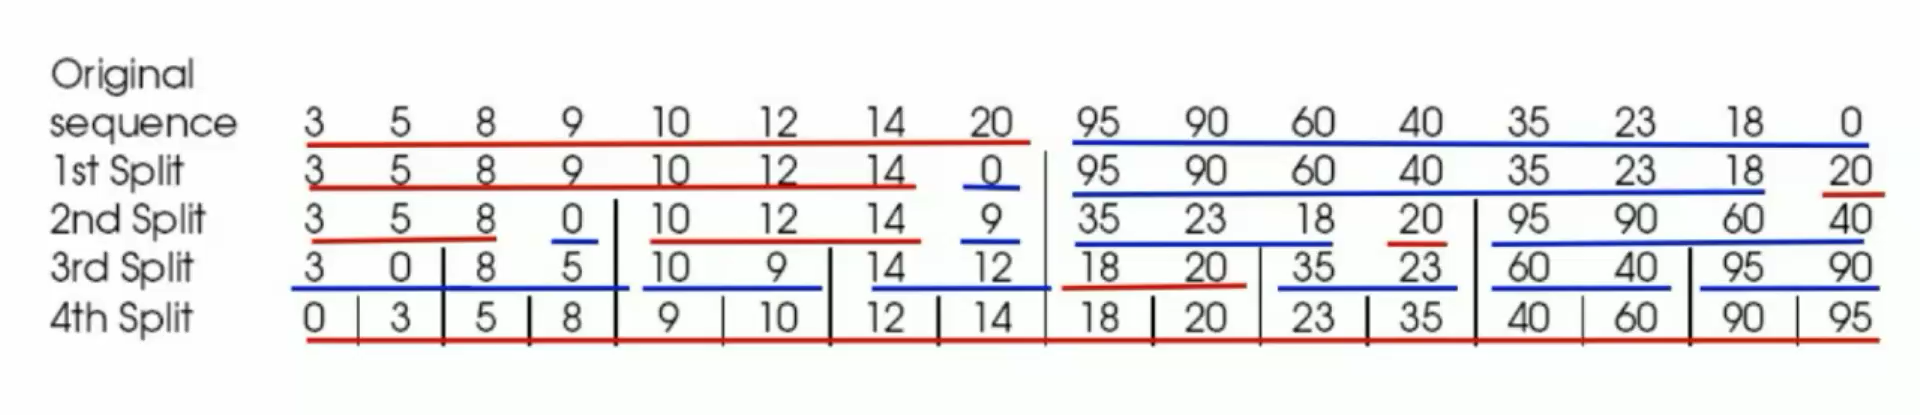
\includegraphics[scale=0.27]{fig1.png}

\paragraph{Analysis.} \textsc{bitonicsort} is oblivious because the behavior of the algorithm does not depend on the content of the input, i.e., the sequence of comparisons is deterministic regardless of the comparison results. At each layer of the recursion, the total number of comparisons made by all calls in this layer is upper bounded by $n/2$. The depth of the recursion is given by \[D(n)  = D(n/2) + \log n \] which solves to $\log n (\log n+1)/2$. Therefore the total number of comparisons is upper bounded by $n/2 \cdot \log n (\log n+1)/2 = \mathcal{O}(n \log^2 n)$, where the Big-O notation hides a relatively small constant.

\section{Bucket Oblivious Sort \cite{bucket}}

We start by introducing the Bucket Oblivious Sorting algorithm that has an $\mathcal{O}(n\log n (\log\log n)^2)$ complexity. Afterward, we will discuss the improvement to speed it up to $\mathcal{O}(n\log n)$. In general, the framework of BucketSort is as follows: 

$ $

\begin{mdframed}[innertopmargin=5pt, skipabove=\topskip, skipbelow=\topskip,align=left]


Given a sequence $A$:
\begin{enumerate}
    \item Apply an \textbf{oblivious random permutation} (\textsc{ORP}) on $A$ to get $A' \gets \textsc{ORP}(A)$.
    \item Sort $A'$ using any (potentially non-oblivious) comparison-based sorting algorithm, e.g. QuickSort.
\end{enumerate}
\end{mdframed}

$ $

As the name suggested, the specification of \textsc{ORP} is that given a sequence $A$, outputs a randomly permuted version of $A$. The obliviousness guarantee is that the access pattern should reveal nothing about the applied random permutation. Our plan is to construct $\textsc{ORP}$ as a randomized algorithm with a \emph{deterministic access pattern}.

\begin{nonexample}
    The Fisher–Yates shuffle is not an oblivious random permutation. It works as follows: Given $A := [A_0, \cdots, A_{n-1}]$,
    \begin{itemize}
        \item for $i \in [0, n-1)$:
        \subitem - $j \rsmpl  [i, n)$;
        \subitem - Swap($A_i$, $A_j$);
    \end{itemize}
    Apparently, one can exactly learn the random permutation applied by observing the Swap instructions. 
\end{nonexample}

\begin{remark}
    It is crucial that in the second step of the BucketSort framework, the sorting algorithm needs to be comparison-based. For example, we cannot use a counting-based sort because even after the sequence is randomly permuted, applying a counting sort would reveal the frequency of elements in each bin, which is exactly what we want to hide. In contrast, a comparison-based sorting will only reveal the relative order between elements, which is fine after we randomly permuted the positions of elements.
\end{remark}

\subsection{Oblivious Random Permutation}

For the purpose of construction \textsc{ORP}, we are going to assign each element to a random bin and then route the elements through a butterfly network to their assigned random bins. A visualization of the network is given on the next page. The behavior of the algorithm is as follows:
\begin{itemize}
    \item (Set-up): Let $Z$ be a size of buckets (which we will choose later as a function of $n$). Let $B := 2n/Z$ be the number of buckets. Each bucket is going to contain $Z/2$ \emph{real} elements from the input sequence and $Z/2$ dummy elements.

    \item Each element is randomly  assigned to one of the $B$ buckets indexed by a key of  $\log B$ bits.

    \item The elements are routed to their respective destinations through a butterfly network, which contains $\log B$ layers that are connected through \textsc{mergesort} operators.

    \item The \textsc{mergesort} operator takes two buckets from the $i^{\text{th}}$ level as inputs and reorganize their elements into two buckets for  the $(i+1)^{\text{th}}$ layer, according to the $(i+1)^{\text{th}}$ most significant bit of the elements' keys. i.e., At the $i^{\text{th}}$ level, every $2i$ consecutive buckets are \emph{semi-sorted} by the most significant $i$ bits of the keys.

    \item Finally, to obtain a random permutation from our random bin assignments, we  simply remove  all  dummy  elements in each bin and then randomly permute each single bucket at the final layer. 
\end{itemize}

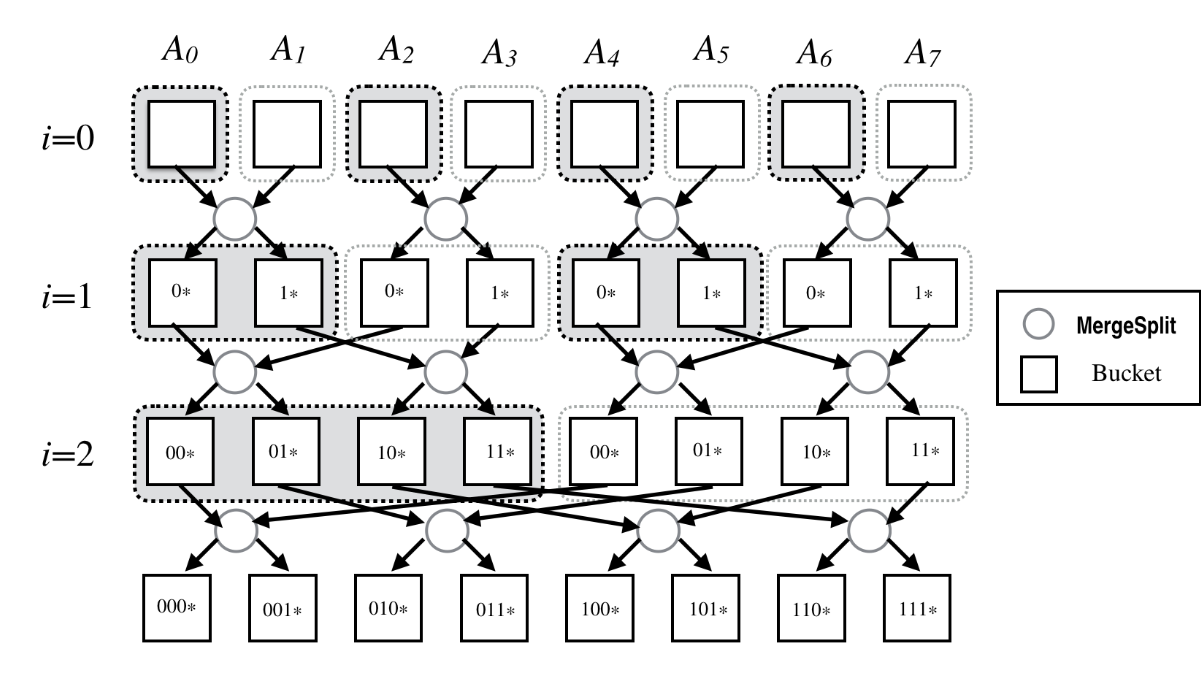
\includegraphics[scale=0.45]{fig2.png}

\paragraph{Efficiency for Clients with $2Z$ storage.}

If the client has a storage size no less than $2Z$, then they can perform \textsc{mergesort} and random permute the buckets at the final layer locally. In each of the $\log B = \log \frac{2n}{Z} < \log N$ layers, the $2n$-sized sequence (containing $n$ real elements and $n$ dummy elements) is read  and written once. So oblivious bin assignment and bucket ORP run in $4n\log n$ time. 

\paragraph{Efficiency for Clients with constant storage.}

With constant-storage clients, we need to implement oblivious \textsc{MergeSplit} using \textsc{bitonicsort}. This is done by sorting the real elements with respect to the keys and then padding each of the resulting buckets with dummy elements. In the final layer, the bucket-wise permutation is also done with \textsc{bitonicsort}. Given a bucket, we firstly assign  each  element  with a  $\log n$-bit label. We then obliviously  sort  the  elements  by  their  labels using  \textsc{bitonicsort}.  In total, at each of the $\log B$ layers, we invoke $B/2$ instances of bitonic sort on $2Z$ elements, thus the  runtime  is  roughly  \[\log B\cdot B/2\cdot 2Z\log^2(2Z))\approx 2n\log n\log^2Z.\]

\paragraph{Success Probability.} The above algorithm is guaranteed to output a correct, randomly permuted version of the input sequence if none of the buckets ever overflows (i.e., receives more than $Z$ real elements) during the routing.

\begin{lemma}
    Overflow happens  with  at most $\epsilon(n,Z) =2n/Z\cdot\log(2n/Z)\cdot e^{-Z/6}$ probability.
\end{lemma}

\begin{proof}
    Consider a bucket $B_i$ at level $i$ which has an associated $i$-bit long prefix $b$ of keys. $B_i$ receives real  elements from $2^i$ initial buckets in the first layer,  each  containing $Z/2$ real  elements. By the construction, any of these elements reaches $B_i$ only if the most significant $i$ bits  of its  key match $b$, which happens with exactly $2^{-i}$ probability. 
    
    A Chernoff bound  shows that $B_i$ overflows  with  less  than $e^{-Z/6}$ probability. Hence, taking a union  bound  over  all  levels and all buckets, we get that overflow happens with less than $\epsilon(n,Z) := B\cdot \log B\cdot e^{-Z/6}$ probability.
\end{proof}



